\newpage

\section{IP Spoofing with Hping3}

\subsection{Activity}

\noindent {\bf{Bước 1:}} Vào \textbf{VirtualBox}. Chọn Windows Server được tạo từ phần 1. Sau đó cài đặt Network thành \textbf{NAT Network}.

\begin{figure}[!htb]
    \centering
    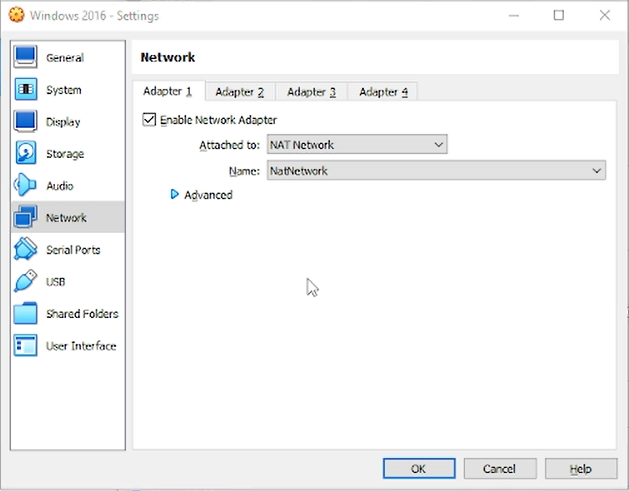
\includegraphics[width=0.7\linewidth]{figure//chapter5//lab5_1/nat_network.png}
    \caption{Cài đặt NAT Network}
    \label{fig:enter-label}
\end{figure}

\noindent Thực hiện tương tự với Kali Linux VM được tạo từ phần 1.

\noindent {\bf{Bước 2:}} Khởi động Windows Server, chọn \textbf{Start} và chọn \textbf{Control Panel}. Chọn \textbf{Ethernet} > \textbf{Properties}. 

\begin{figure}[!htb]
    \centering
    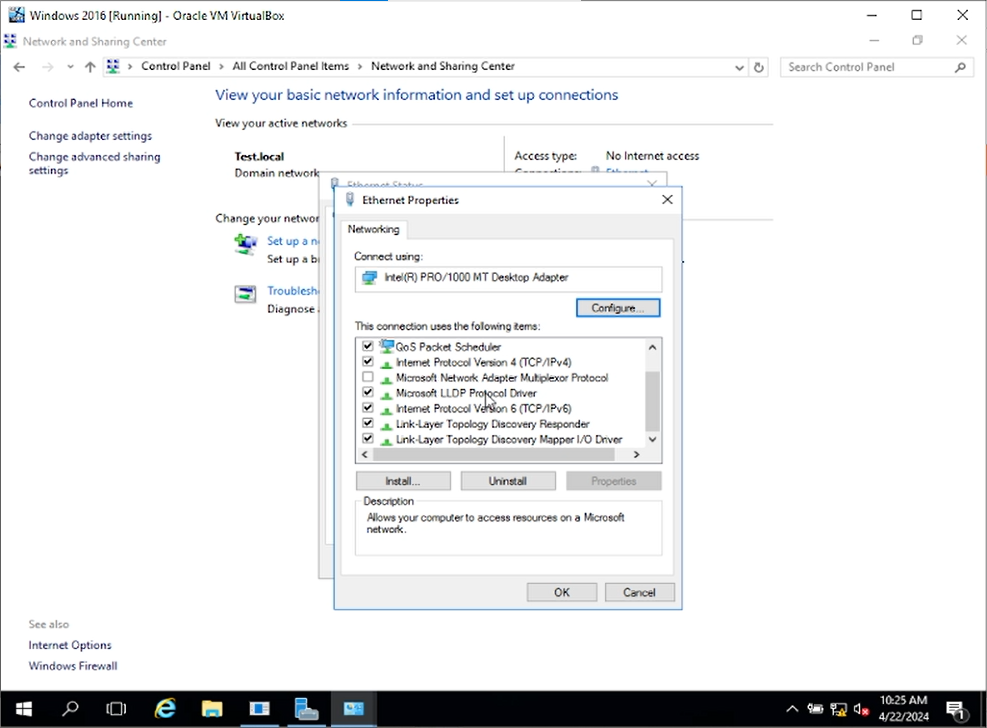
\includegraphics[width=0.7\linewidth]{figure//chapter5//lab5_2/ethernet_properties.png}
    \caption{Ethernet Properties}
    \label{fig:enter-label}
\end{figure}

\newpage

\noindent {\bf{Bước 3}} Chọn \textbf{Internet Protocol Version 4} > Properties. 

\begin{figure}[!htb]
    \centering
    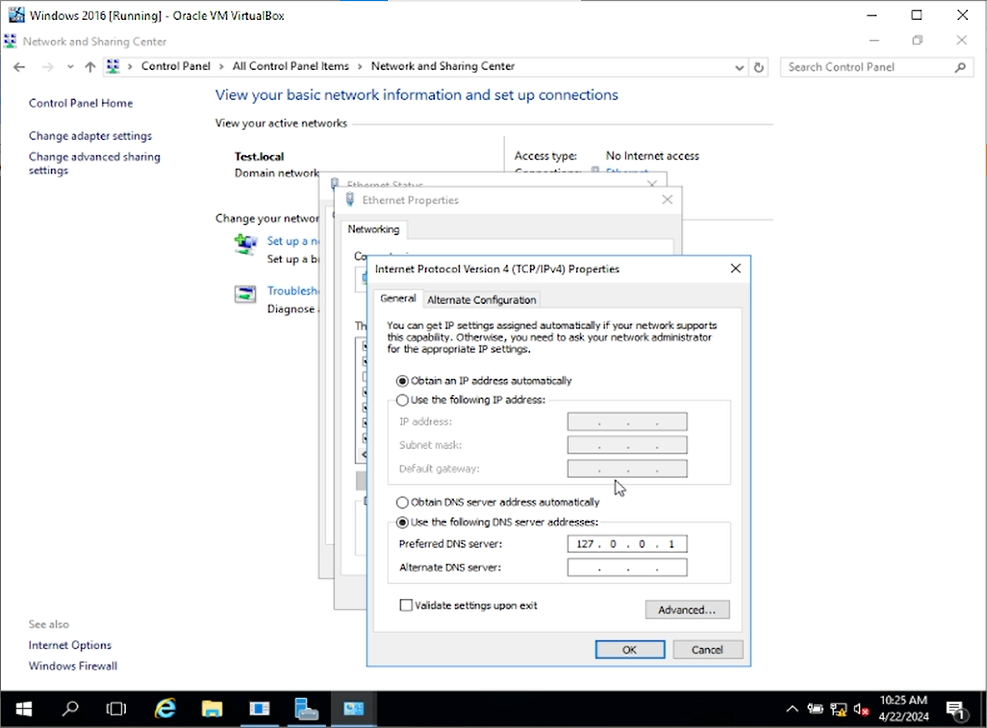
\includegraphics[width=0.85\linewidth]{figure//chapter5//lab5_2/ipv4_properties.png}
    \caption{IPv4 Properties}
    \label{fig:enter-label}
\end{figure}

\noindent {\bf{Bước 4}} Điền IP 192.168.0.1 và subnet mask 255.255.255.0.

\begin{figure}[!htb]
    \centering
    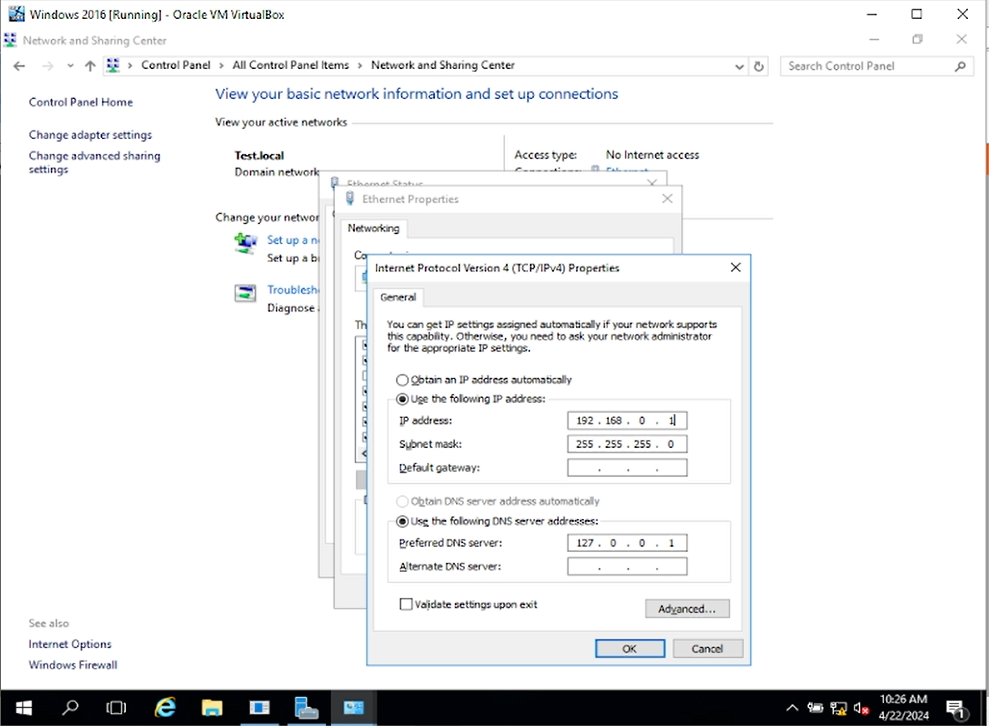
\includegraphics[width=0.85\linewidth]{figure//chapter5//lab5_2/configure_ip.png}
    \caption{Cấu hình IPv4}
    \label{fig:enter-label}
\end{figure}

\newpage

\noindent {\bf{Bước 5}} Tạo một Windows 10 VM khác giống hệt với Windows Server. Sau đó, cấu hình mạng tương tự với các bước trên, chỉ thay bằng địa chỉ IP 192.168.0.2.

\begin{figure}[!htb]
    \centering
    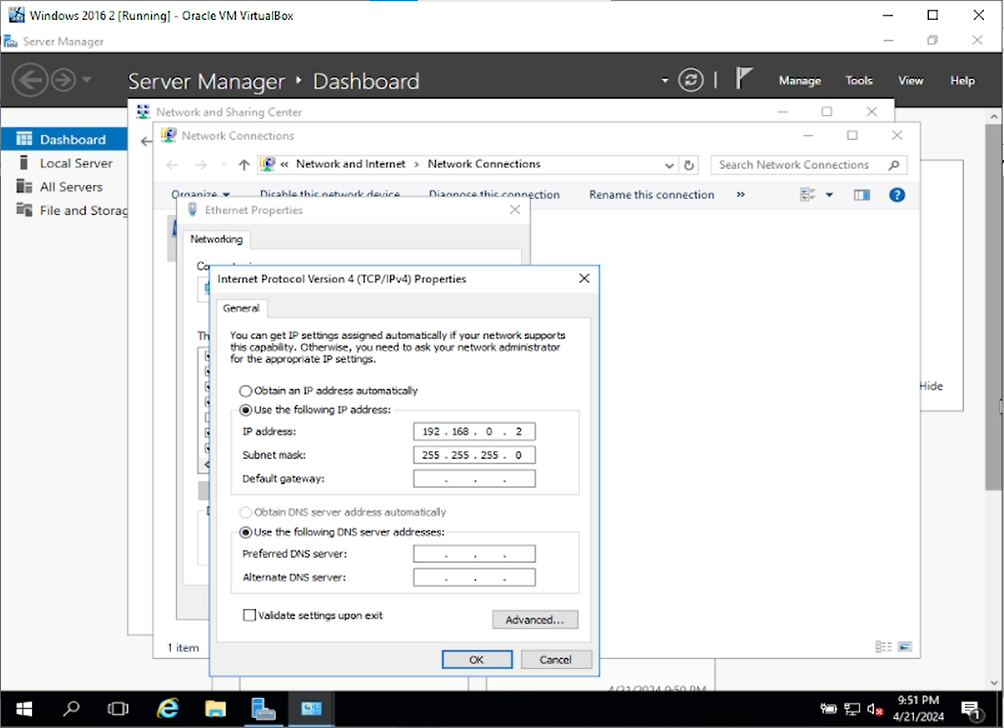
\includegraphics[width=0.85\linewidth]{figure//chapter5//lab5_2/windows10_network.png}
    \caption{Cấu hình mạng Windows 10}
    \label{fig:enter-label}
\end{figure}

\noindent {\bf{Bước 6}} Ở Kali Linux VM, chọn \textbf{Show application} và chọn \textbf{Settings}.

\begin{figure}[!htb]
    \centering
    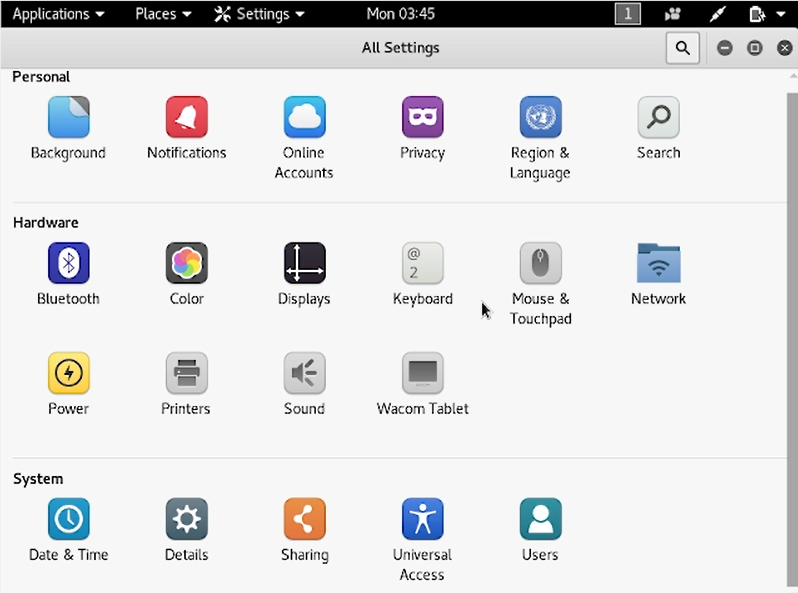
\includegraphics[width=0.85\linewidth]{figure//chapter5//lab5_2/setting-linux.png}
    \caption{Màn hình Settings của Kali Linux VM}
    \label{fig:enter-label}
\end{figure}

\noindent {\bf{Bước 7}} Chọn Network để cấu hình mạng. Tại \textbf{TPv4}, đặt IP là 192.168.0.3 và subnet mask là 255.255.255.0.

\begin{figure}[!htb]
    \centering
    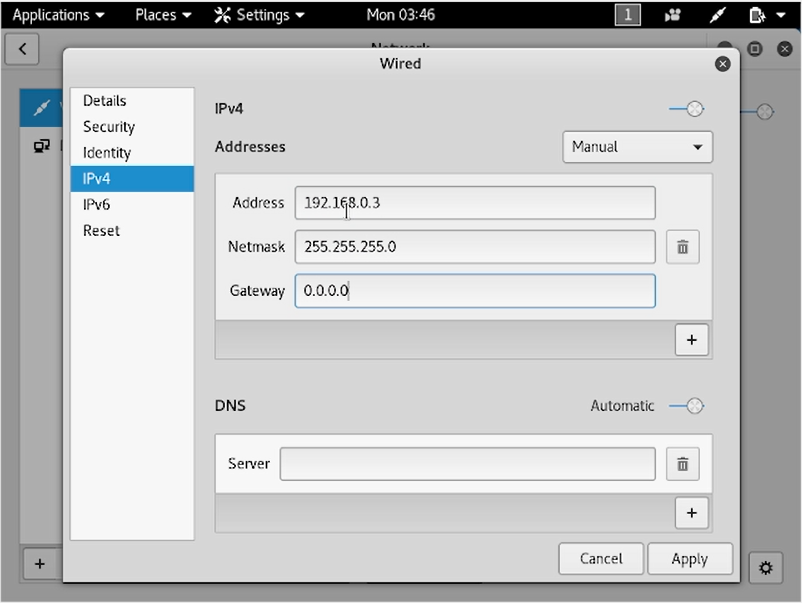
\includegraphics[width=0.85\linewidth]{figure//chapter5//lab5_2/network-linux.png}
    \caption{Cấu hình mạng trên Kali Linux}
    \label{fig:enter-label}
\end{figure}

\noindent {\bf{Bước 8}} Mở \textbf{Terminal} và nhập \textbf{hping3 --help} để biết thêm thông tin của lệnh này.

\begin{figure}[!htb]
    \centering
    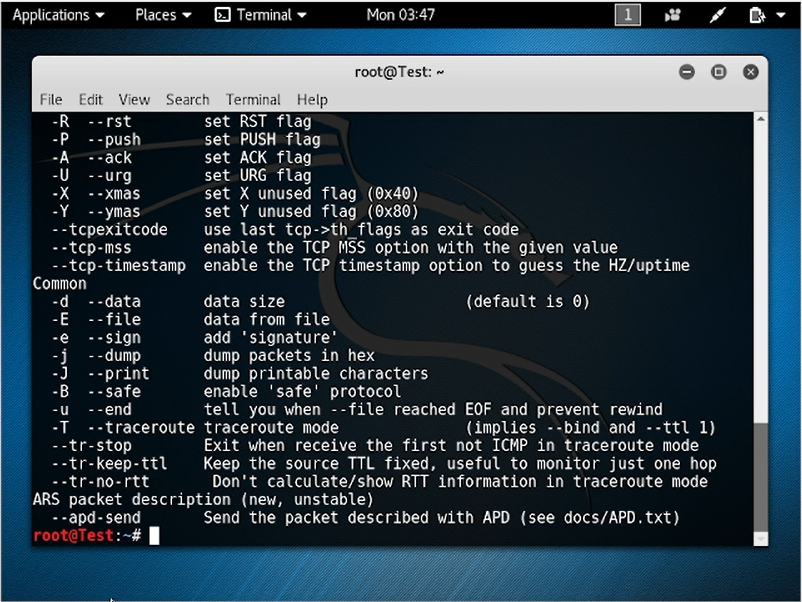
\includegraphics[width=0.8\linewidth]{figure//chapter5//lab5_2/hping3_info.png}
    \caption{Thông tin lệnh hping3}
    \label{fig:enter-label}
\end{figure}

\noindent {\bf{Bước 9}} Nhập \textbf{wireshark} để mở ứng dụng WireShark. Bạn có thể gặp một cảnh báo thì hãy chọn \textbf{OK}.

\begin{figure}[!htb]
    \centering
    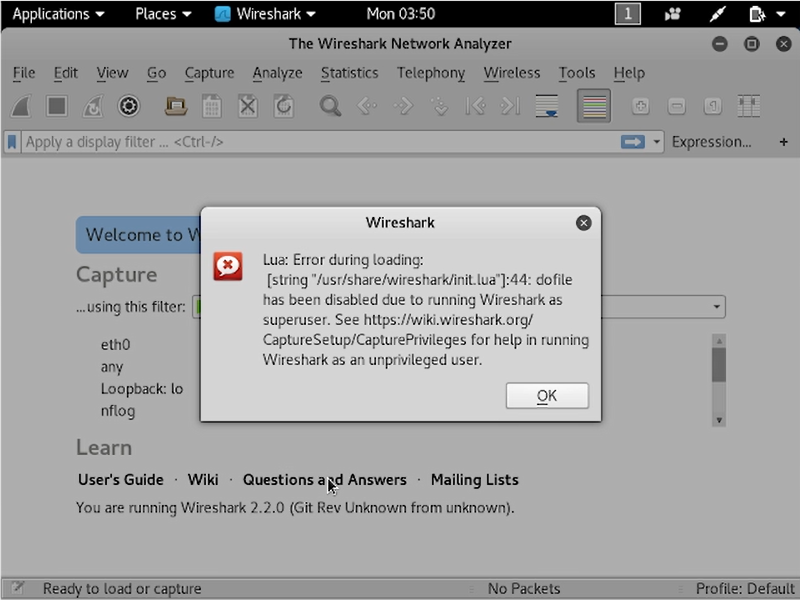
\includegraphics[width=0.8\linewidth]{figure//chapter5//lab5_2/wireshark.png}
    \caption{Màn hình và cảnh báo từ WireShark}
    \label{fig:enter-label}
\end{figure}

\noindent {\bf{Bước 10}} Ở \textbf{Terminal}, nhập \textbf{hping3 -s 192.168.0.1} để ping tới Windows Server VM.

\begin{figure}[!htb]
    \centering
    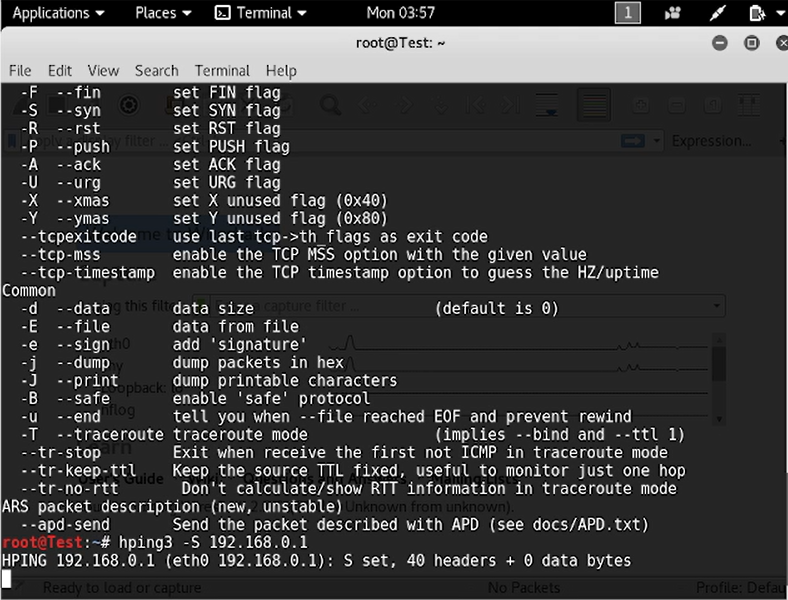
\includegraphics[width=0.8\linewidth]{figure//chapter5//lab5_2/ping_to_windows_server.png}
    \caption{Ping tới máy ảo Windows Server}
    \label{fig:enter-label}
\end{figure}

\newpage

\noindent {\bf{Bước 11}} Quay lại WireShark, chọn \textbf{etho} và nhấn \textbf{Click/Start}. Đợi 10s rồi \textbf{Stop}. Bạn có thể thấy các thông báo khi có packet gửi tới cho Windows Server VM.

\begin{figure}[!htb]
    \centering
    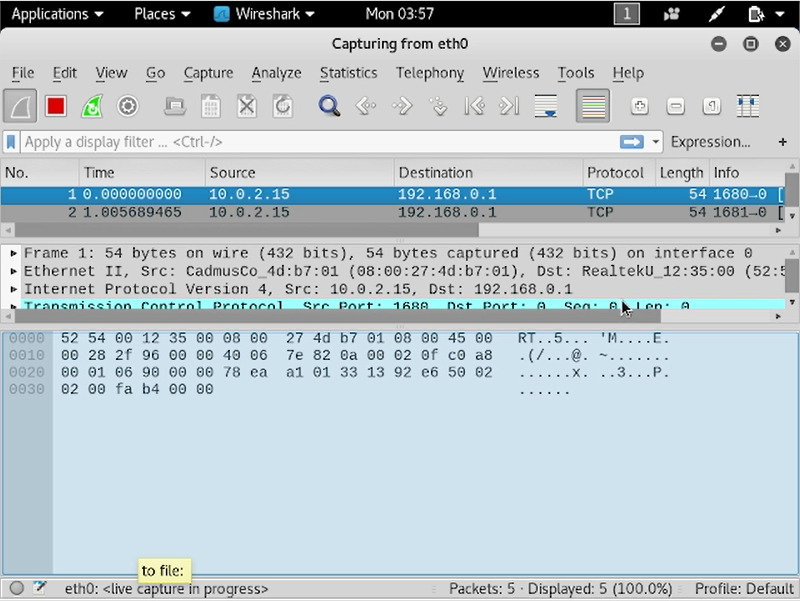
\includegraphics[width=0.8\linewidth]{figure//chapter5//lab5_2/capture_wireshark.png}
    \caption{Màn hình Wireshark khi Capture}
    \label{fig:enter-label}
\end{figure}

\noindent {\bf{Bước 12}} Tiếp theo, bạn sẽ tiến hành gửi các packet tới cho Windows Server từ Kali Linux, nhưng do đang giả mạo IP nên hệ thống sẽ hiện nguồn từ Windows 10 VM thay vì Kali Linux. Chạy \textbf{hping3 -S 192.168.0.2 -a 192.168.0.1}

\begin{figure}[!htb]
    \centering
    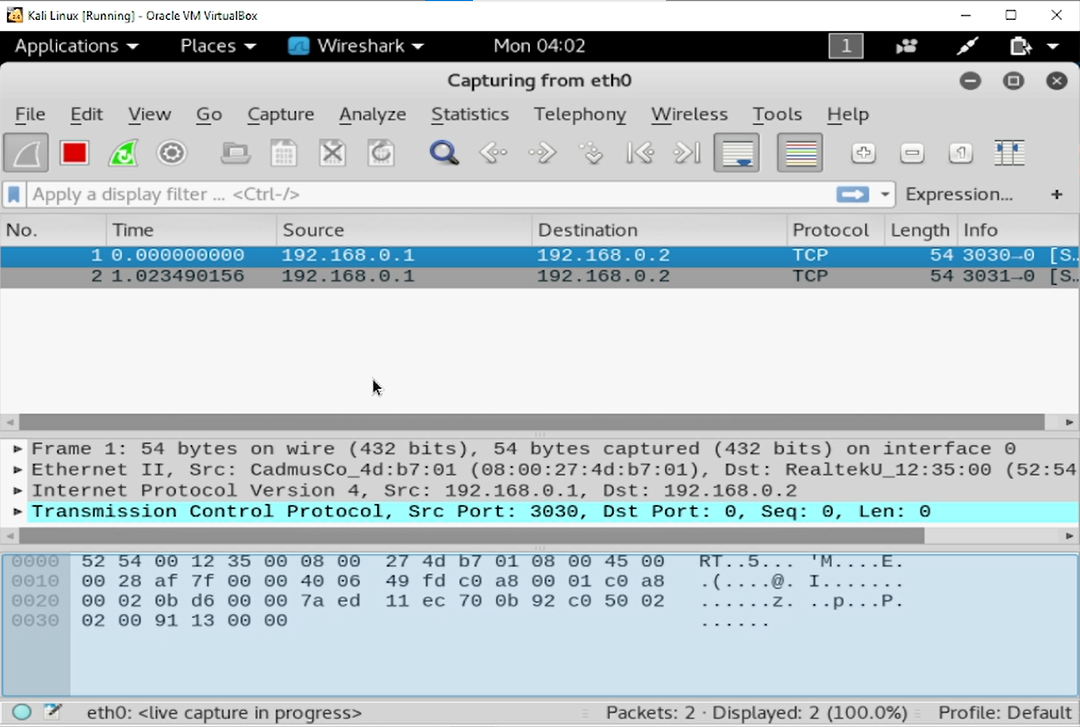
\includegraphics[width=0.8\linewidth]{figure//chapter5//lab5_2/spoof.png}
    \caption{Kết quả khi thay đổi địa chỉ IP}
    \label{fig:enter-label}
\end{figure}

\subsection{Review Questions}

\noindent Câu 1: Because it is absent from back table.

\noindent Câu 2: UDP.

\noindent Câu 3: 

A: Clicking the frame, expanding the Transmission Control Protocol node in the middle frame, and seeing that the Flags item lists (RST).

\noindent Câu 4:

A: -f.

\noindent Câu 5:

C: -K.

